\subsection{Proof Procedure}.  
   
   \begin{figure}[htb]
    \centering
		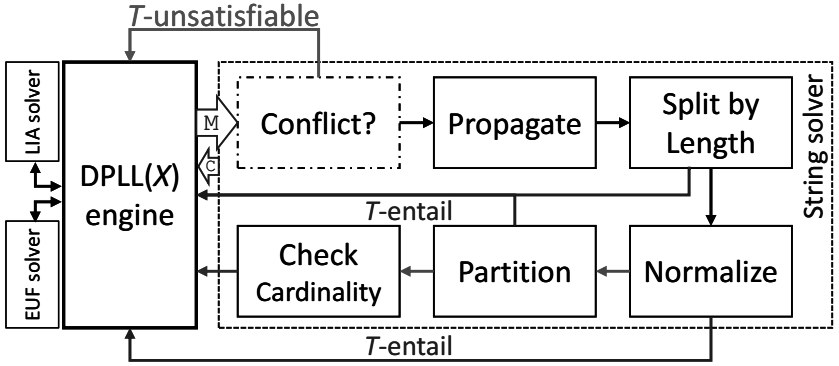
\includegraphics[width=0.7\linewidth]{pictures/proof_procedure.png}
	\caption{Abstracted core proof procedure for string. The figure is taken from \cite{main_phd}.}
	\label{fig:proof_procedure}
	\end{figure}
	
	
	In this section, we will see how the derivation rules are applied to produce the derivation tree. According to the authors of paper \cite{main-paper} this proof procedure is a highly abstracted version of the one which is implemented in cvc4 string solver. The main procedure is based on the repeated application of the rules according to the seven steps below (also as shown in Figure \ref{fig:proof_procedure}). In cases of split, the left branch configuration is tried first. The procedure interrupts and restarts with Step 0 as soon as new constraint is introduced to $S$. The procedure keeps cycling through the steps until it derives a configuration where no rules applies or the \texttt{unsat} one. In the case of \texttt{unsat}, if there is other branch configuration, the procedure continues with that branch in the derivation tree.

\begin{description}			
	\item$Step\ 0:$ $Reset:$ Apply \texttt{Reset} to reset buckets, and flat and normal forms.
	\item$Step\ 1:$ $Check\ for\ conflicts:$ Apply \texttt{S-Conflict} or \texttt{A-Conflict} if the configuration is unsatisfiable due to the current string or arithmetic constraints.
	\item$Step\ 2:$ $Propagate:$ Apply \texttt{S-Prop} and \texttt{A-Prop} and propagate entailed equalities between $S$ and $A$.
	\item$Step\ 3:$  $Add\ length\ constraints:$ For each non-variable $t \in \mathcal{T}(S)$, apply \texttt{Len} to add the equality $ \texttt{len}(x)\approx \texttt{len}(t)$ to \texttt{A}.  For each variable $x$ in $\mathcal{V}(S \cup A)$, apply \texttt{Len-Split},and then first explore the branch where $x \approx \epsilon$.
	\item$Step\ 4:$ $Compute\ Normal\ Forms\ for\ Equivalence\ Classes:$ Apply \texttt{S-Cycle} to shrinks concatenation terms. Then apply the normalization rules \texttt{F-Form1},\texttt{F-Form2}, \texttt{N-Form1} and \texttt{N-Form2} to completion. The idea is to produce a total map $N$. If not, then rules like \texttt{L-Split}, \texttt{F-Unify}, \texttt{F-Split}, \texttt{F-loop} are applied according to different cases. Detail on this can be found on paper \cite{main_phd}.
		
	\item$Step\ 5: Partition\ equivalence\ classes\ into\ buckets:$ The target is to distribute each equivalence class to a bucket. First apply \texttt{D-Base} and \texttt{D-Add} to completion. This should make $B$ a partition of \( \textnormal{E}_S \). If not, then there is an equivalence class $[x]$ which is not contained in any bucket. At this step rules like \texttt{S-Split}, \texttt{D-Split}, \texttt{L-Split} are applied according to different cases. Detail on this can be found on paper \cite{main_phd}.
	\item$Step\ 6:Add\ length\ constraint\ for\ cardinality:$ Apply the rule \texttt{Card} for each bucket. This will introduce new arithmetic constraints corresponding to the minimal length of terms in $B$ based on the number of equivalence classes in $B$ and the cardinality $| \mathcal{A}|$ of the alphabet. For instance, if $\Sigma$ is a finite alphabet of 256 characters and $S$ entails that 257 distinct strings of length 1 exist, then $S$ is unsatisfiable. 
\end{description}
    In this section, we have presented a brief and abstract overview of the procedure. The description of the different steps are taken from \cite{main_phd}. In the subsequent section we will present few examples of the application of the derivation according to this procedure.
